\chapter{Processing Models}

\section{Motivation}
\begin{definitionbox}{Processing Model}
    A mechanism used to connect operators acting on data in a query.
    \begin{itemize}
        \item Choice is critical to database design.
    \end{itemize}
\end{definitionbox}

\begin{definitionbox}{Function Objects}
    References to code that can be passed, invoked, change state and produce values.
    \begin{minted}{cpp}
#include <functional>

std::function<int(int, int)> add = [ /* captures */ ](int a, int b) { return a + b; }
    \end{minted}
    See \href{https://en.cppreference.com/w/cpp/language/lambda}{C++11 Lambdas}
    \begin{itemize}
        \item Can capture variables (value and references to) (also called closures).
        \item Used to implement single abstract method classes in some languages (e.g kotlin, java)
    \end{itemize}
\end{definitionbox}

\section{Volcano Processing}
\begin{definitionbox}{Volcano Processing Model}
    \begin{center}
        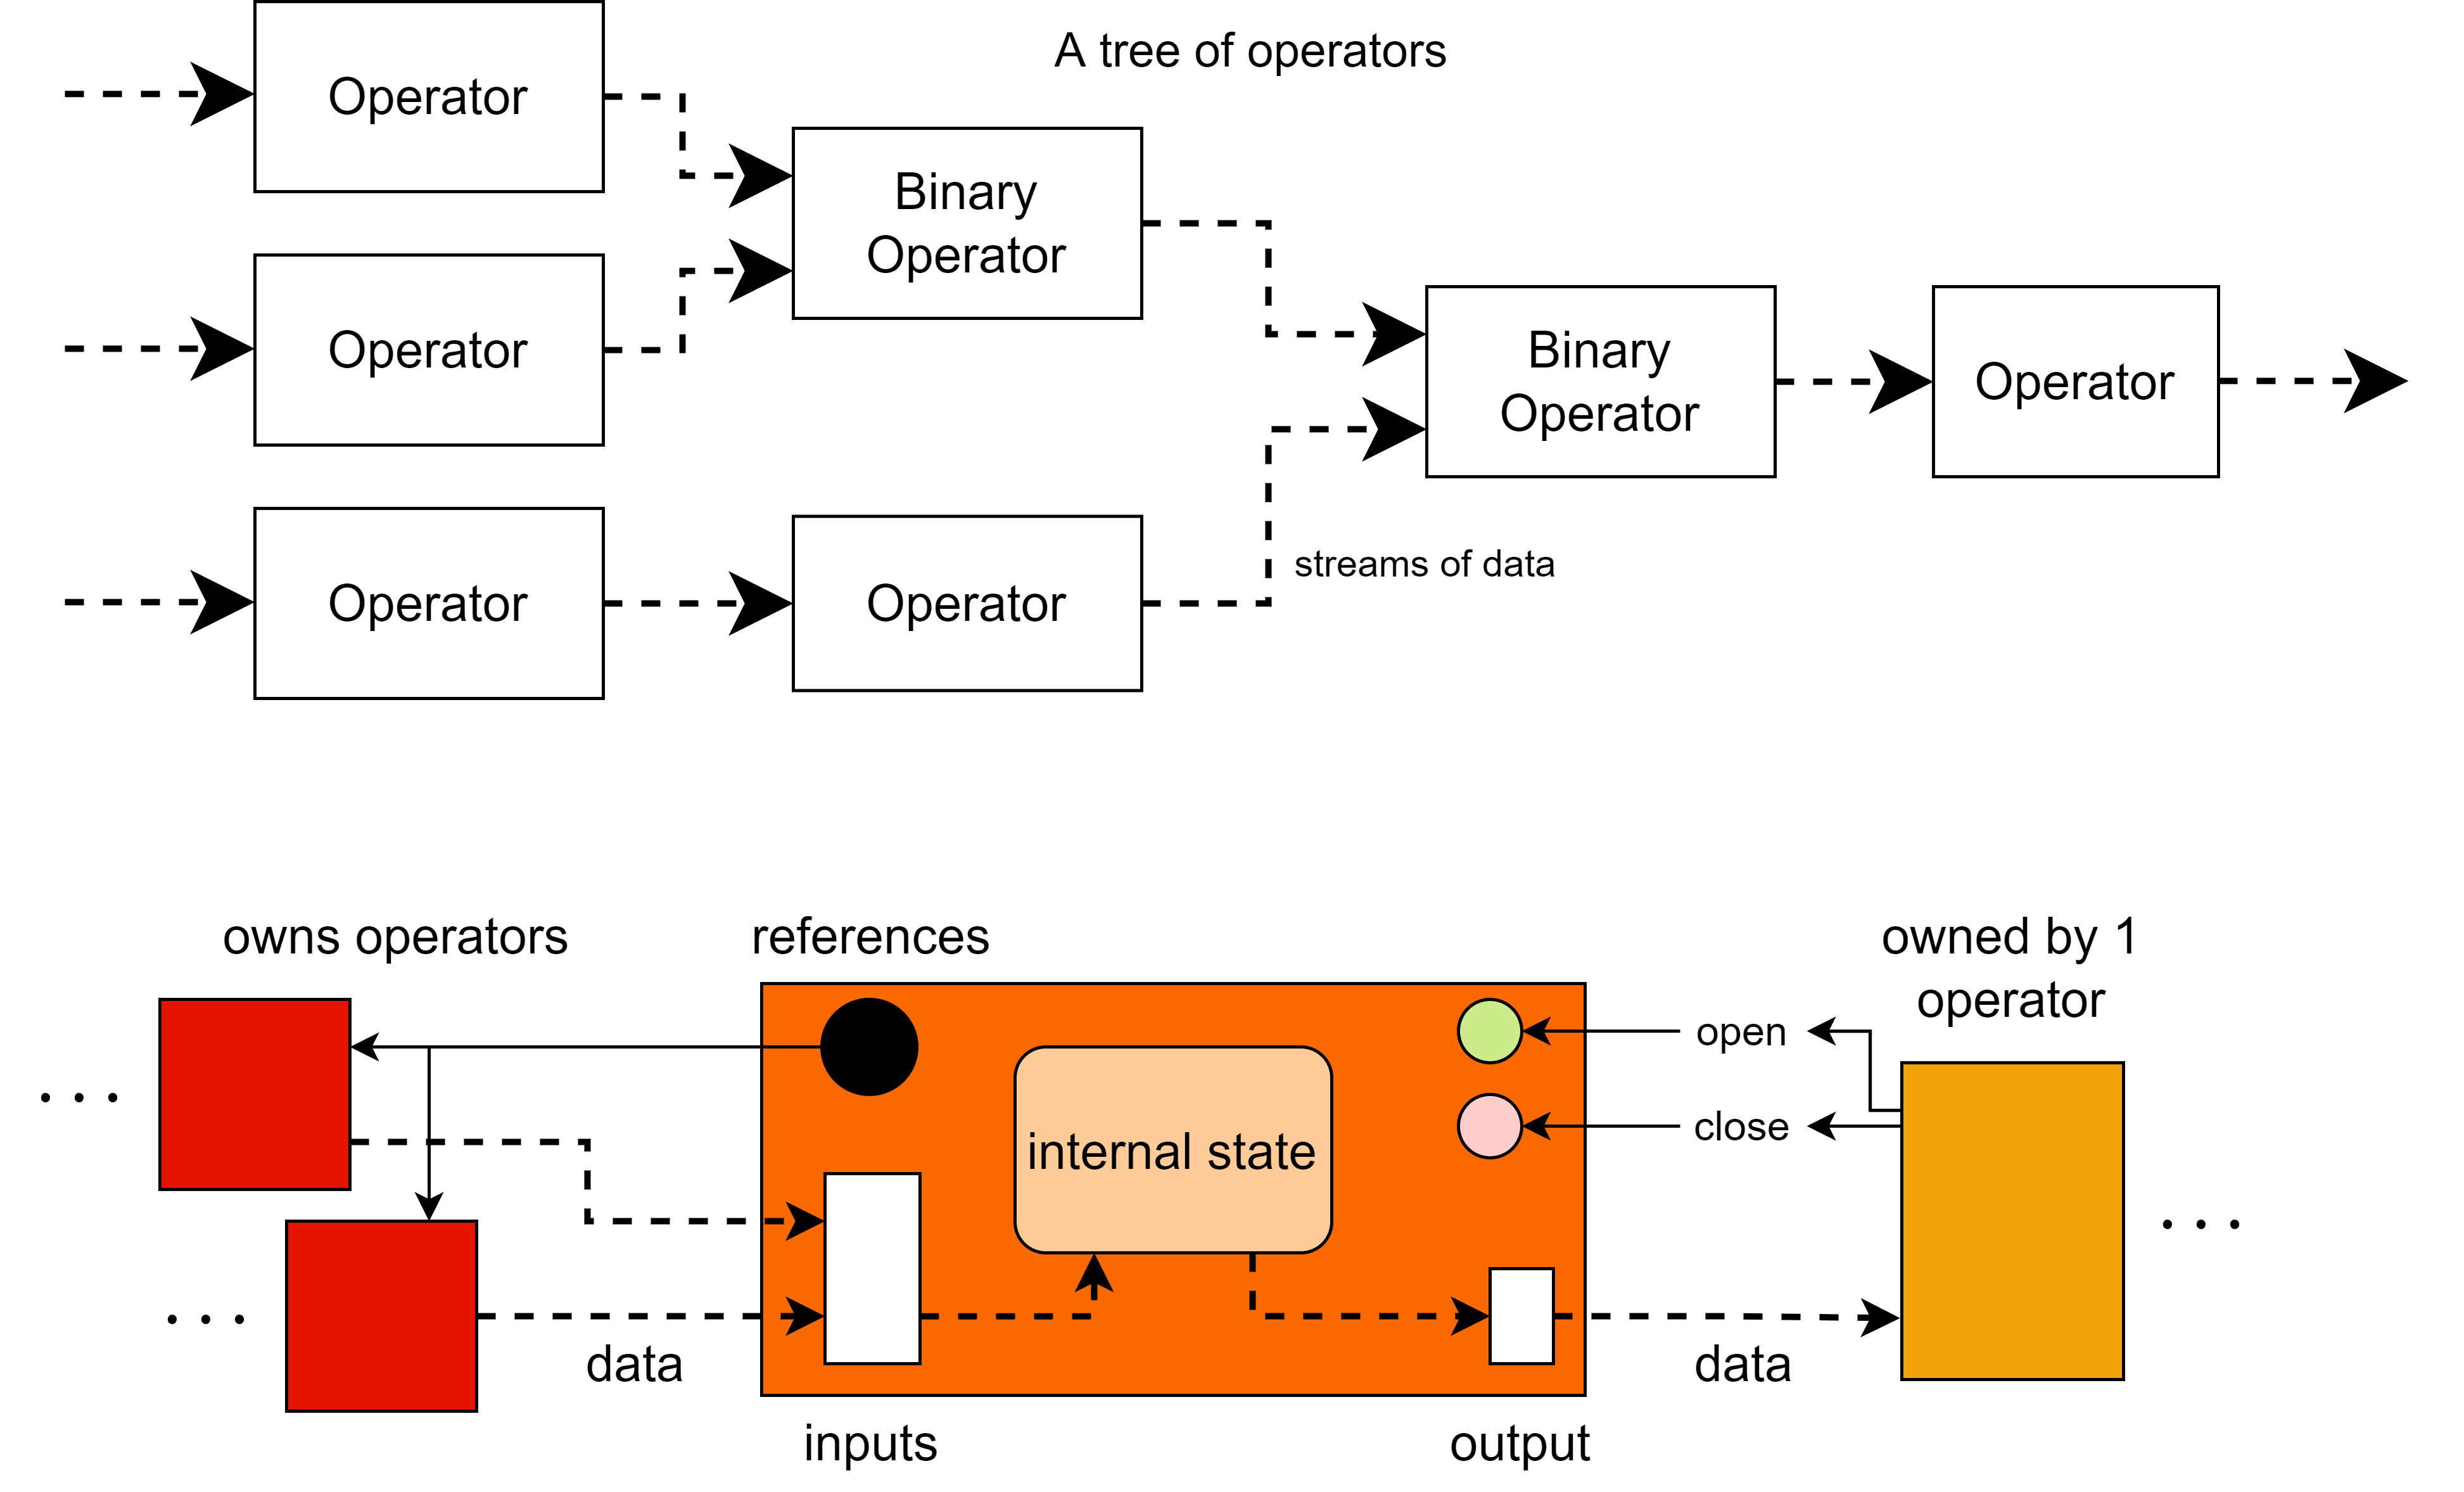
\includegraphics[width=.9\textwidth]{processing_models/images/volcano_stages.drawio.png}
    \end{center}
    Data is fed chunk by chunk (row) through a tree of operators.
    \begin{itemize}
        \item Older design (influential in the 80s) with a focus on design practices over performance. At the time this was an alternative to ad-hoc implementation.
        \item Uses non-relational physical algebra (specialized to be useful in expressing queries for a physical plan, rather than as an abstraction for the programmer).
    \end{itemize}
\end{definitionbox}

\begin{tabbox}{prosbox}
  \textbf{Easy to Implement} & Implementation is simple, adding new operators is easy (using operator interface provided). Clean Object-Oriented Design. \\
  \textbf{I/O Behaviour} & As tuples are consumed as soon as they are produced, no waiting for I/O to create and buffer the next tuple. \\
\end{tabbox}
\begin{tabbox}{consbox}
  \textbf{Lots of Calls!} & CPU spends much time loading and calling function pointers to operators, predicates and aggregate functions. \\
\end{tabbox}

\subsection{Operators}
A basic interface for operators can be devised as:
\begin{minted}{cpp}
template <typename T>
struct Operator
{
  virtual void open() = 0;
  virtual void close() = 0;
  virtual optional<T> next() = 0;
};
\end{minted}
In order to allow the greatest flexibility in using our operators, they are parameterised by \mintinline{cpp}{typename T}. 
In the concrete examples this is set as a \textit{runtime tracked} type \mintinline{cpp}{Row} which is variable size, and contains variants of \mintinline{cpp}{int}, \mintinline{cpp}{char}, \mintinline{cpp}{bool}, etc.
\\
\\ We could also swap this out for a reference, or pointer to some \textit{runtime type} to avoid copying.

\begin{sidenotebox}{But why not RAII}
    To keep these examples explicit, an \mintinline{cpp}{open()} and \mintinline{cpp}{close()} are overriden, rather than using the constructor \& destructor.
    \\
    \\ That said RAII would be useful here:
    \begin{itemize}
        \item Automatically clean up after operators after they are dropped.
        \item Cannot be used before open/construction, or used after close/destruction.
    \end{itemize}
\end{sidenotebox}

\subsubsection{Scan}
Scans a table already loaded into memory to return its rows.
\begin{minted}{cpp}
template <typename T>
struct Scan : Operator<T>
{
  using TableType = vector<T>;
  /* Many different operators can have a reference to and read the table.
   * - shared_ptr drops table after it is no longer needed
   * - must avoid copying very large table structure
   */
  Scan(shared_ptr<TableType> t) : _table(t), _index(0) { assert(_table); }

  /* No operation on open / close */
  void open() override {}
  void close() override {}

  optional<T> next() override
  {
    if (_index < (*_table).size())
    {
      return (*_table)[_index++];
    }
    else
    {
      return {};
    }
  }

private:
  shared_ptr<TableType> _table;
  size_t _index;
};
\end{minted}

\subsubsection{Project}
\begin{minted}{cpp}
template <typename T, typename S>
struct Project : Operator<T>
{
  using Projection = function<T(S)>;

  Project(unique_ptr<Operator<S>> child, Projection proj)
      : _child(move(child)), _proj(proj)
  {
    assert(_child);
  }

  void open() override { _child->open(); }
  void close() override { _child->close(); }

  optional<T> next() override
  {
    // Note: can be simplified with optional<A>::and_then(function<B(A)>) in C++23
    auto next = _child->next();
    if (next.has_value())
    {
      return _proj(next.value());
    }
    else
    {
      return {};
    }
  }

private:
  unique_ptr<Operator<S>> _child;
  Projection _proj;
};
\end{minted}

\subsubsection{Select}
\begin{minted}{cpp}
template <typename T>
struct Select : Operator<T>
{
  using Predicate = function<bool(T)>;

  Select(unique_ptr<Operator<T>> child, Predicate pred)
      : _child(move(child)), _pred(pred)
  {
    assert(_child);
  }

  void open() override { _child->open(); }
  void close() override { _child->close(); }

  optional<T> next() override
  {
    auto candidate = _child->next();
    // keep getting candidates until there are no more, or one is valid.
    while (candidate.has_value() && !_pred(candidate.value()))
    {
      candidate = _child->next();
    }
    return candidate;
  }

private:
  unique_ptr<Operator<T>> _child;
  Predicate _pred;
};
\end{minted}

\subsubsection{Union}
\begin{minted}{cpp}
template <typename T>
struct Union : Operator<T>
{
  Union(unique_ptr<Operator<T>> leftChild, unique_ptr<Operator<T>> rightChild)
      : _leftChild(move(leftChild)), _rightChild(move(rightChild))
  {
    assert(_leftChild && _rightChild);
  }

  void open() override
  {
    _leftChild->open();
    _rightChild->open();
  }
  void close() override
  {
    _leftChild->close();
    _rightChild->close();
  }

  optional<T> next() override
  {
    auto candidate = _leftChild->next();
    if (candidate.has_value())
    {
      return candidate;
    }
    else
    {
      return _rightChild->next();
    }
  }

private:
  unique_ptr<Operator<T>> _leftChild, _rightChild;
};
\end{minted}

\subsubsection{Difference}

\begin{definitionbox}{Pipeline Breaker}
    An operator which can only produce its first value/output tuple after all inputs from one or more input operators has been processed.
    \begin{itemize}
        \item Usually requires some kind of buffering (e.g with \mintinline{cpp}{Difference}).
    \end{itemize}
\end{definitionbox}

Difference breaks the pipeline as we need to know all tuples from one side (the subtracting set) before we can start to produce rows.

\begin{minted}{cpp}
/* The definition of difference forces the pipeline to be broken (buffering) */
template <typename T>
struct Difference : Operator<T>
{
  Difference(unique_ptr<Operator<T>> fromChild,
             unique_ptr<Operator<T>> subChild)
      : _fromChild(fromChild), _subChild(subChild), _subBuffer()
  {
    assert(_fromChild && _subChild);
  }

  void open() override
  {
    _fromChild->open();
    _subChild->open();

    // buffer all to subtract
    for (auto candidate = _subChild->next(); candidate.has_value();
         candidate = _subChild->next())
    {
      _subBuffer.push_back(candidate);
    }
  }
  void close() override
  {
    _fromChild->close();
    _subChild->close();
  }

  optional<T> next() override
  {
    auto candidate = _fromChild->next();
    // keep getting next until there is no next candidate, or the candidate is
    // not being subtracted
    while (candidate.has_value() && _subBuffer.contains(candidate.value()))
    {
      candidate = _fromChild->next();
    }
    return candidate;
  }

private:
  unique_ptr<Operator<T>> _fromChild, _subChild;
  unordered_set<T> _subBuffer;
};
\end{minted}

\subsubsection{Cartesian/Cross Product}
This can be optionally implemented as a \textit{pipeline breaker}.

\begin{minted}{cpp}

template <typename A, typename B>
struct BreakingCrossProduct : Operator<tuple<A, B>>
{
  BreakingCrossProduct(unique_ptr<Operator<A>> leftChild,
                       unique_ptr<Operator<B>> rightChild)
      : _leftChild(move(leftChild)), _rightChild(move(rightChild)),
        _leftCurrent(), _rightIndex(0), _rightBuffer()
  {
    assert(_leftChild && _rightChild);
  }

  void open() override
  {
    _leftChild->open();
    _rightChild->open();

    // set first left (can be none -> in which case next will never return
    // anything)
    _leftCurrent = _leftChild->next();

    // buffer in the entirety of the right
    for (auto candidate = _rightChild->next(); candidate.has_value();
         candidate = _rightChild->next())
    {
      _rightBuffer.push_back(candidate.value());
    }
  }

  void close() override
  {
    _leftChild->close();
    _rightChild->close();
  }

  optional<tuple<A, B>> next() override
  {
    // invariant: _rightBuffer.size() > _rightIndex >= 0
    if (_leftCurrent.has_value() && !_rightBuffer.empty())
    {
      auto next_val =
          make_tuple(_leftCurrent.value(), _rightBuffer[_rightIndex]);

      _rightIndex++;
      if (_rightIndex == _rightBuffer.size())
      {
        _rightIndex = 0;
        _leftCurrent = _leftChild->next();
      }

      return next_val;
    }
    else
    {
      return {};
    }
  }

private:
  unique_ptr<Operator<A>> _leftChild;
  unique_ptr<Operator<B>> _rightChild;
  optional<A> _leftCurrent;
  size_t _rightIndex;
  vector<B> _rightBuffer;
};
\end{minted}
A Non-pipeline breaking implementation has two phases:
\begin{enumerate}
    \item Collecting rows from the right child operator, while using the same row from the left.
    \item The right child operator has been exhausted, slowly get tuples from the left while traversing tuples collected from the right.
\end{enumerate}
\begin{minted}{cpp}
template <typename A, typename B>
struct CrossProduct : Operator<tuple<A, B>>
{
  CrossProduct(unique_ptr<Operator<A>> leftChild,
               unique_ptr<Operator<B>> rightChild)
      : _leftChild(move(leftChild)), _rightChild(move(rightChild)),
        _leftCurrent(), _rightBuffered(), _rightOffset(0)
  {
    assert(_leftChild && _rightChild);
  }

  void open() override
  {
    _leftChild->open();
    _rightChild->open();
    _leftCurrent = _leftChild->next();
  }
  void close() override
  {
    _leftChild->close();
    _rightChild->close();
  }

  optional<tuple<A, B>> next() override
  {
    /* invariants:
     * - _leftCurrent is already set
     * - if there are no more _rightChild to get, then we are iterating over the
     *   _leftChild
     */
    auto rightCandidate = _rightChild->next();
    if (rightCandidate.has_value())
    {
      // still getting content from the right had side
      _rightBuffered.push_back(rightCandidate.value());
    }
    else if (_rightOffset == _rightBuffered.size())
    {
      // all tuples have been taken from right hand side, now using buffer
      _leftCurrent = _leftChild->next();
      _rightOffset = 0;
    }

    // only return if both sides have values
    if (_leftCurrent.has_value() && !_rightBuffered.empty())
    {
      // get tuple and increment _rightOffset
      return make_tuple(_leftCurrent.value(), _rightBuffered[_rightOffset++]);
    }
    else
    {
      return {};
    }
  }

private:
  unique_ptr<Operator<A>> _leftChild;
  unique_ptr<Operator<B>> _rightChild;
  optional<A> _leftCurrent;
  vector<B> _rightBuffered;
  size_t _rightOffset;
};
\end{minted}

\subsubsection{Group Aggregation}
This is fundamentally a \textit{pipeline breaker}, and must buffer rows prior to \mintinline{cpp}{next()}. 
The algorithm acts in three phases:
\begin{enumerate}
    \item Buffer tuples from the child.
    \item Get the key (column being grouped by e.g \mintinline{SQL}{GROUP BY column1}) and aggregation (e.g \mintinline{SQL}{SELECT MAX(column2)}) and place in a hashmap.
    \item Finally provide rows through \mintinline{cpp}{next()}
\end{enumerate}
\begin{minted}{cpp}
/* We use the template to determine the hash and nextSlot implementations used
 * T        -> type of data provided by the child
 * S        -> data output by the groupBy & aggregation
 * K        -> the type grouped on, produced by a grouping function (K group(T))
 * hash     -> a function to convert a key into a hash
 * nextSlot -> to determine next slot in collisions
 */
 template <typename T, typename S, typename K, size_t nextSlot(size_t),
          size_t hashFun(K), size_t OVERALLOCATE_FACTOR = 2>
struct GroupBy : Operator<S>
{
  using Aggregation = function<S(optional<S>, T)>;
  using Grouping = function<K(T)>;

  GroupBy(unique_ptr<Operator<T>> child,
          Grouping grouping,
          Aggregation aggregation) : _child(move(child)), _grouping(grouping),
                                     _aggregation(aggregation), _hashTable(), _hashTableCursor(0)
  {
    assert(_child);
  }

  void open() override
  {
    _child->open();

    vector<T> childValues;
    for (auto currentVal = _child->next();
         currentVal.has_value();
         currentVal = _child->next())
    {
      childValues.push_back(currentVal.value());
    }

    _hashTable = vector<optional<pair<K, S>>>(childValues.size(), optional<pair<K, S>>());
    for (T val : childValues)
    {
      K key = _grouping(val);
      size_t slot = hashFun(key) % _hashTable.size();
      while (_hashTable[slot].has_value() && _hashTable[slot].value().first != key)
      {
        slot = nextSlot(slot) % _hashTable.size();
      }

      // slot is now correct, either a value present with the same key, or none.
      auto prev_val = _hashTable[slot].has_value() ? _hashTable[slot].value().second : optional<S>();
      _hashTable[slot] = optional<pair<K, S>>(make_pair<K, S>(move(key), _aggregation(prev_val, val)));
    }

    // all values moved into the hashtable, so vector deallocated
  }

  void close() override
  {
    _child->close();
  }

  optional<S> next() override
  {
    while (_hashTableCursor < _hashTable.size())
    {
      auto slot = _hashTable[_hashTableCursor];
      _hashTableCursor++;

      if (slot.has_value())
      {
        return slot.value().second;
      }
    }
    return {};
  }

private:
  Aggregation _aggregation;
  Grouping _grouping;
  unique_ptr<Operator<T>> _child;
  vector<optional<pair<K, S>>> _hashTable;
  size_t _hashTableCursor;
};
\end{minted}

\subsubsection{Operators Composed}
We can finally define types to use with our operators.
\begin{minted}{cpp}
using Value = variant<int, char, bool>;
using Row = vector<Value>;
using Table = vector<Row>;
\end{minted}
And now build a query from them
\begin{minted}{cpp}
SELECT table.1, MAX(table.0) FROM table GROUP BY table.1;
\end{minted}
\begin{minted}{cpp}
shared_ptr<Table> data = make_shared<Table>(Table{
    {1, 'c', true},
    {1, 'c', false},
    {2, 'c', false},
    {1, 'd', true},
    {3, 'e', false}});

auto scan1 = make_unique<Scan<Row>>(data);
auto scan2 = make_unique<Scan<Row>>(data);
auto cross = make_unique<CrossProduct<Row, Row>>(move(scan1), move(scan2));

Project<Row, tuple<Row, Row>> proj(move(cross), [](tuple<Row, Row> t)
                                    {
  auto vec2 = get<1>(t);
  auto vec1 = get<0>(t);
  vec1.insert(vec1.end(), vec2.begin(), vec2.end());
  return vec1; 
});

GroupBy<Row, Row, Value, nextSlotLinear, hashValue>
    groupby(move(scan), groupBySecondCol, aggregateSecondCol);

groupby.open();
for (auto val = groupby.next(); val.has_value(); val = groupby.next())
{
  cout << val.value() << endl;
}
groupby.close();
\end{minted}

\begin{minted}{bash}
[ 3 e]
[ 5 c]
[ 1 d]
\end{minted}

\begin{sidenotebox}{Run it!}
    The above code is provided with examples in the associated notes repository!
\end{sidenotebox}

\subsection{Pipelining}
\subsubsection{IO Operations}
\begin{center}
  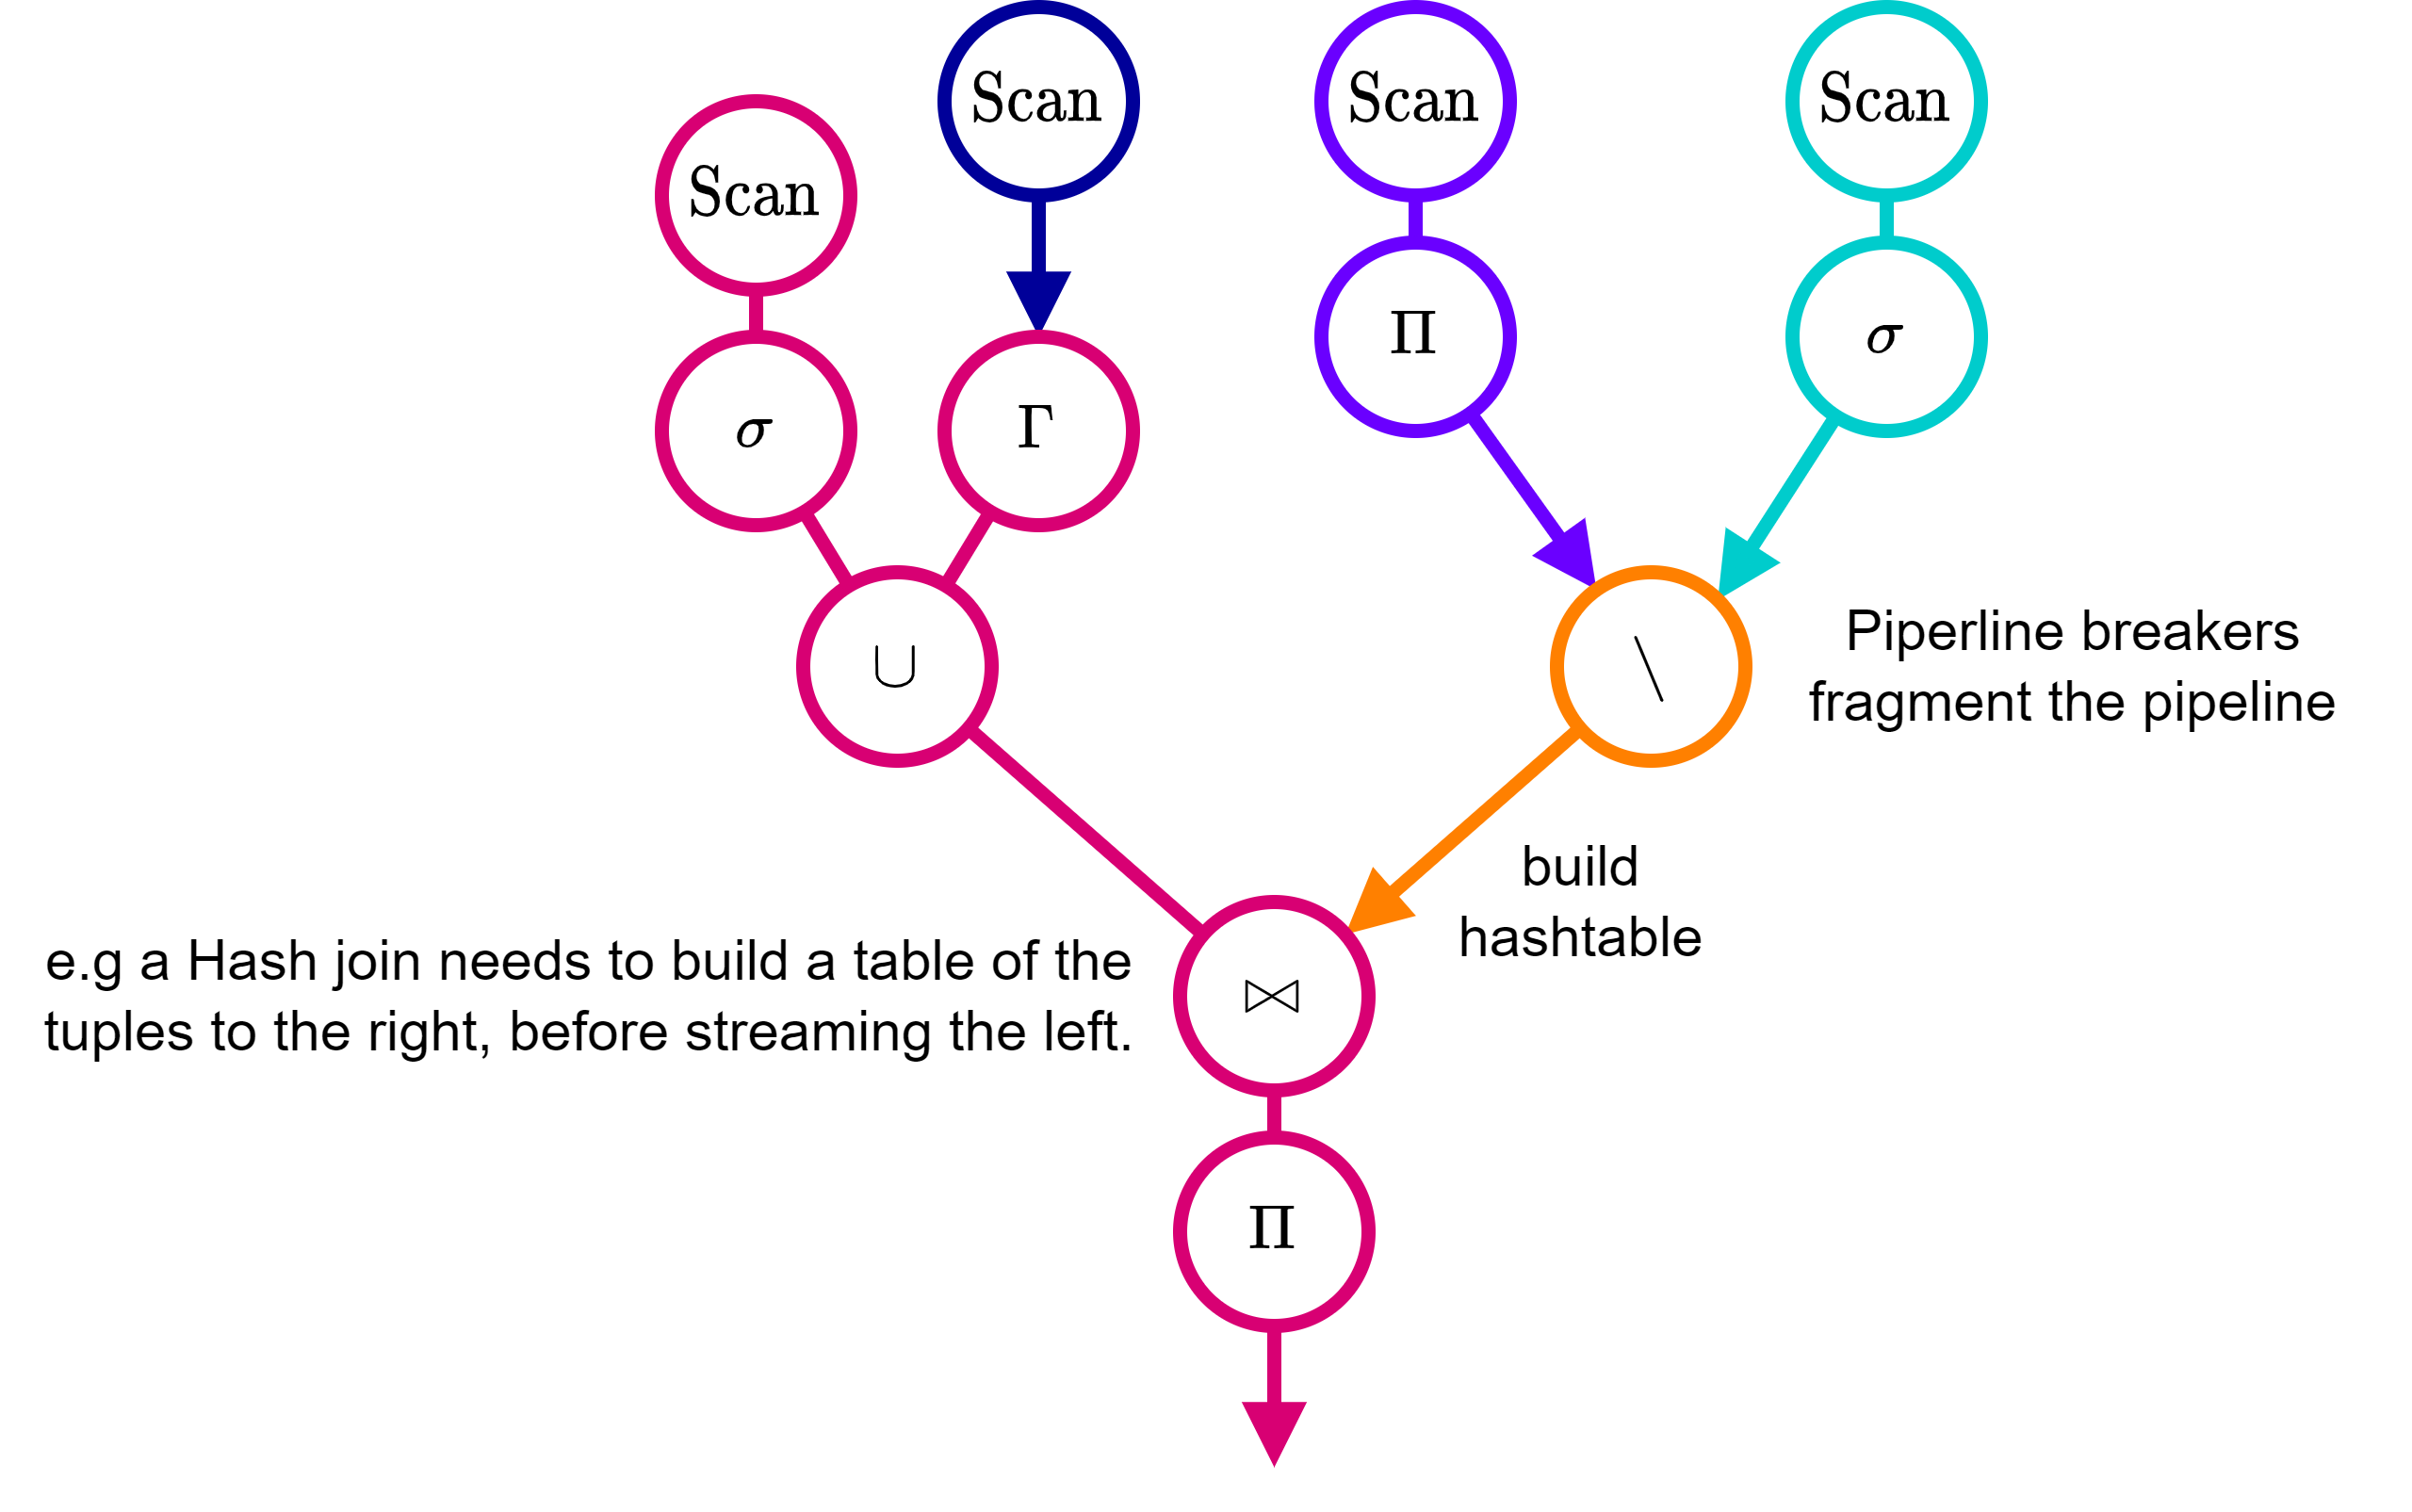
\includegraphics[width=.7\textwidth]{processing_models/images/pipeline_fragments.drawio.png}
\end{center}
As some operations require buffering, we need to determine how much buffer is required, if this can fit in memory (or disk I/O required), and in which operators.
\begin{itemize}
  \item If all buffers in a fragment fit in memory, there is no I/O
  \item Otherwise: sequential access $\to$ number of occupied pages, random access/out of order $\to$ one page I/O per access (an upper bound \& almost certainly an over estimate)
\end{itemize}
Buffer size depends on the operator, we assume \textit{spanned pages} are used:
\begin{itemize}
  \item Sorted relations, nested loop buffers $\to$ same size as input
  \item Hashtables have an over-allocation factor (if not known $\to$ assume $2$)
\end{itemize}
Finally we assume we know the cardinality of operator inputs and outputs, and the buffer pool size.

\begin{examplebox}{Basic GroupBy}
  \begin{minipage}{.2\textwidth}
    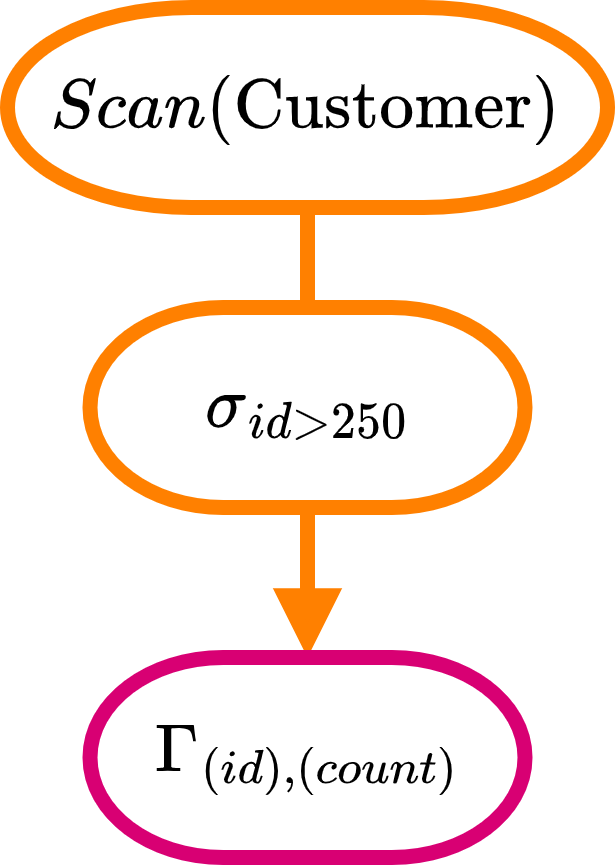
\includegraphics[width=\textwidth]{processing_models/images/example_buffer_io_1.drawio.png}
  \end{minipage} \hfill \begin{minipage}{.79\textwidth}
    \begin{minted}{sql}
CREATE TABLE Customer (
  id      i32,
  name    STRING, -- Key into compressed dictionary
  address STRING, -- Key into compressed dictionary
  nation  i32,
  phone   i32,
  accNum  i32
);
    \end{minted}
    \begin{itemize}
      \item Customer has $10,000$ tuples
      \item Strings are represented by a 32 bit integer key into a compressed dictionary. 
      \item $\sigma_{id > 250}$ has $30\%$ selectivity.
      \item $\Gamma_{(id), (count)}$ has grouping cardinality of $9$
      \item Page size is $64 \ B$
      \item Buffer pool is $512 \ KB$
    \end{itemize}
  \end{minipage}
  \tcblower
  \begin{enumerate}
    \item { $Scan(Customer)$:
      \[size(Customer) = (6 \times 4) \times 10,000 = 240,000 \Rightarrow pages(Customer) = \left\lceil \cfrac{240,000}{64} \right\rceil = 3,750\]
      \begin{itemize}
        \item Scan reads sequentially, so $cost(Scan(Customer)) = 3,750$ I/O operations. 
        \item Not a pipeline-breaker, so only needs 1 tuple at a time, so no buffer allocation required.
      \end{itemize}
    }
    \item { $\sigma_{id < 250}(\dots)$
      \begin{itemize}
        \item Not a pipeline breaker, so no need to buffer.
        \item No IO costs as child $Scan$ operation passes tuple in memory.
      \end{itemize}
    }
    \item { $\Gamma_{(id),(count)}$
      \\ For the grouping we assume a hashtable overallocation factor of $2$, the table contains $count$ and grouping attribute ($id$).
      \[size(\text{GroupBy hashtable}) = 2 \times ((2 \times 4) \times 9) = 144\]
    }
  \end{enumerate}
\end{examplebox}

\subsubsection{CPU Efficiency}
\begin{sidenotebox}{Slow Jumps}
  A jump to a function pointer (e.g a \mintinline{cpp}{std::function}, \mintinline{cpp}{virtual} method or \mintinline{cpp}{OUT (*function_ptr)(A, B, ...)}) is expensive.
  \begin{center}
    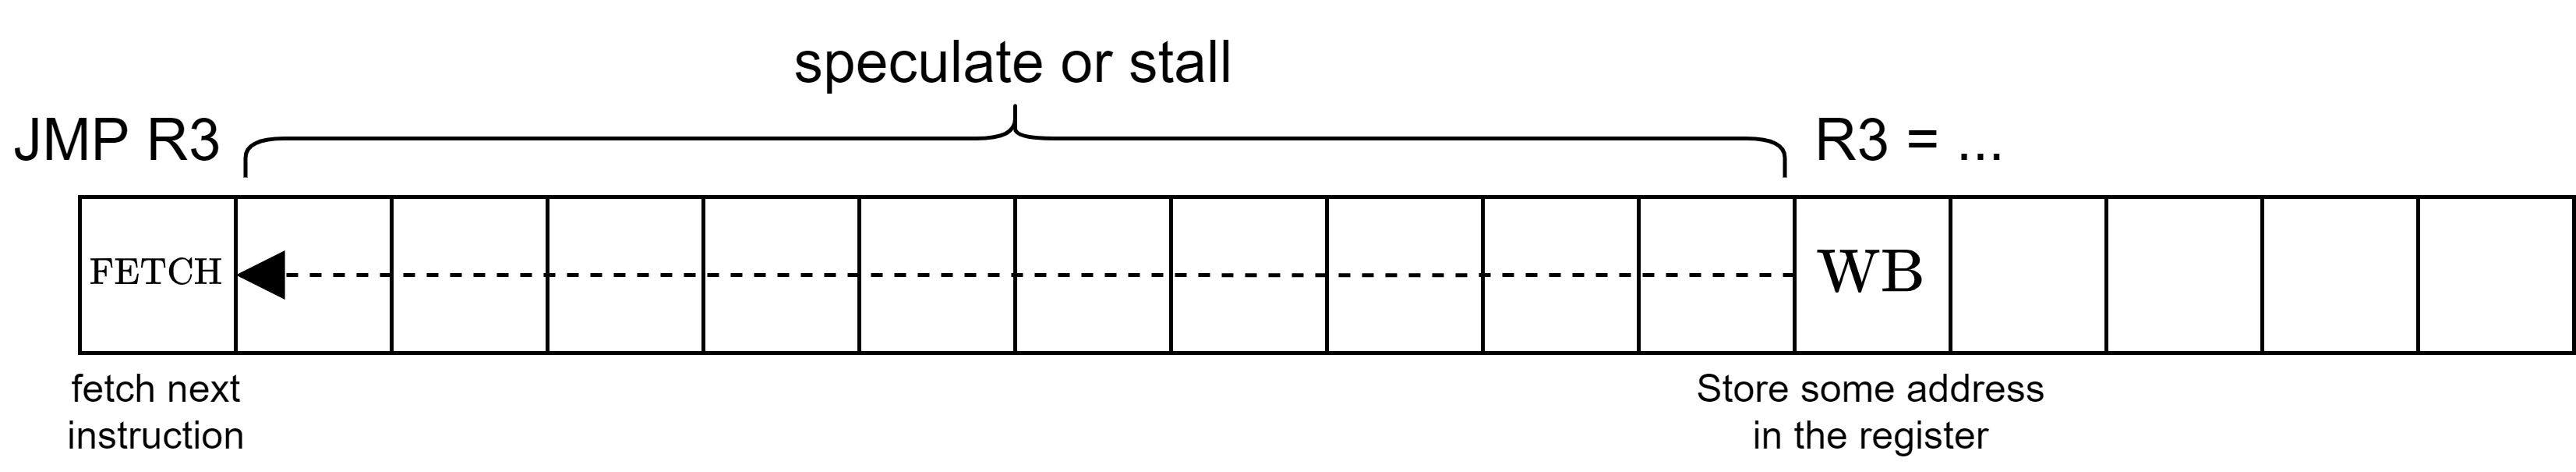
\includegraphics[width=.8\textwidth]{processing_models/images/jump_to_register.drawio.png}
  \end{center}
  \begin{itemize}
    \item A combined data \& control hazard. The address must be known in order to jump, the next instruction after the jump cannot be known until the jump is done.
    \item There are ways to reduce the stall in hardware (reducing length of pipeline frontend to reduce possible stall cycles, jump target prediction \& speculation, delayed jump (allow other work to be done in what would have been stall cycles))
    \item In software we could load the address to a register many instructions before the jump, and do other useful work between, but often there is little other work to be done.
  \end{itemize}
  To avoid this cost:
  \begin{itemize}
    \item Jump to an immediate value (typically pc-relative immediate offset in the jump instruction), as the jump location is part of the instruction, there is no hazard. But the function to jump to must be known at compile time. Still affects returns (jump to link register/return address register) (though this should be very fast due to return-address stack branch predictors).
    \item Inline a function (must be known at compile time)
    \item Do fewer of these calls to function pointers/virtuals.
  \end{itemize}
\end{sidenotebox}
For each operation we can count the function calls per tuple
\begin{center}
  \begin{tabular}{l l p{.6\textwidth}}
    Scan & 0 & Tuples read straight from buffer. \\
    Select/$\sigma$ & 2 & Call to read input, call to apply predicate. \\
    Project/$\Pi$ & 2 & Call to read input, call to projection. \\
    Cross Product (Inner \& Outer) & 1 & Call to read input. \\
    Join & 1 & Call to read input (comparison and hash can be inlined). \\
    Group-By & 2 & Read input and call aggregation function. \\
    Output & 1 & Call to read input and extract to output. \\
   \end{tabular}
\end{center}

\subsection{Operations Calculations}
\begin{center}
  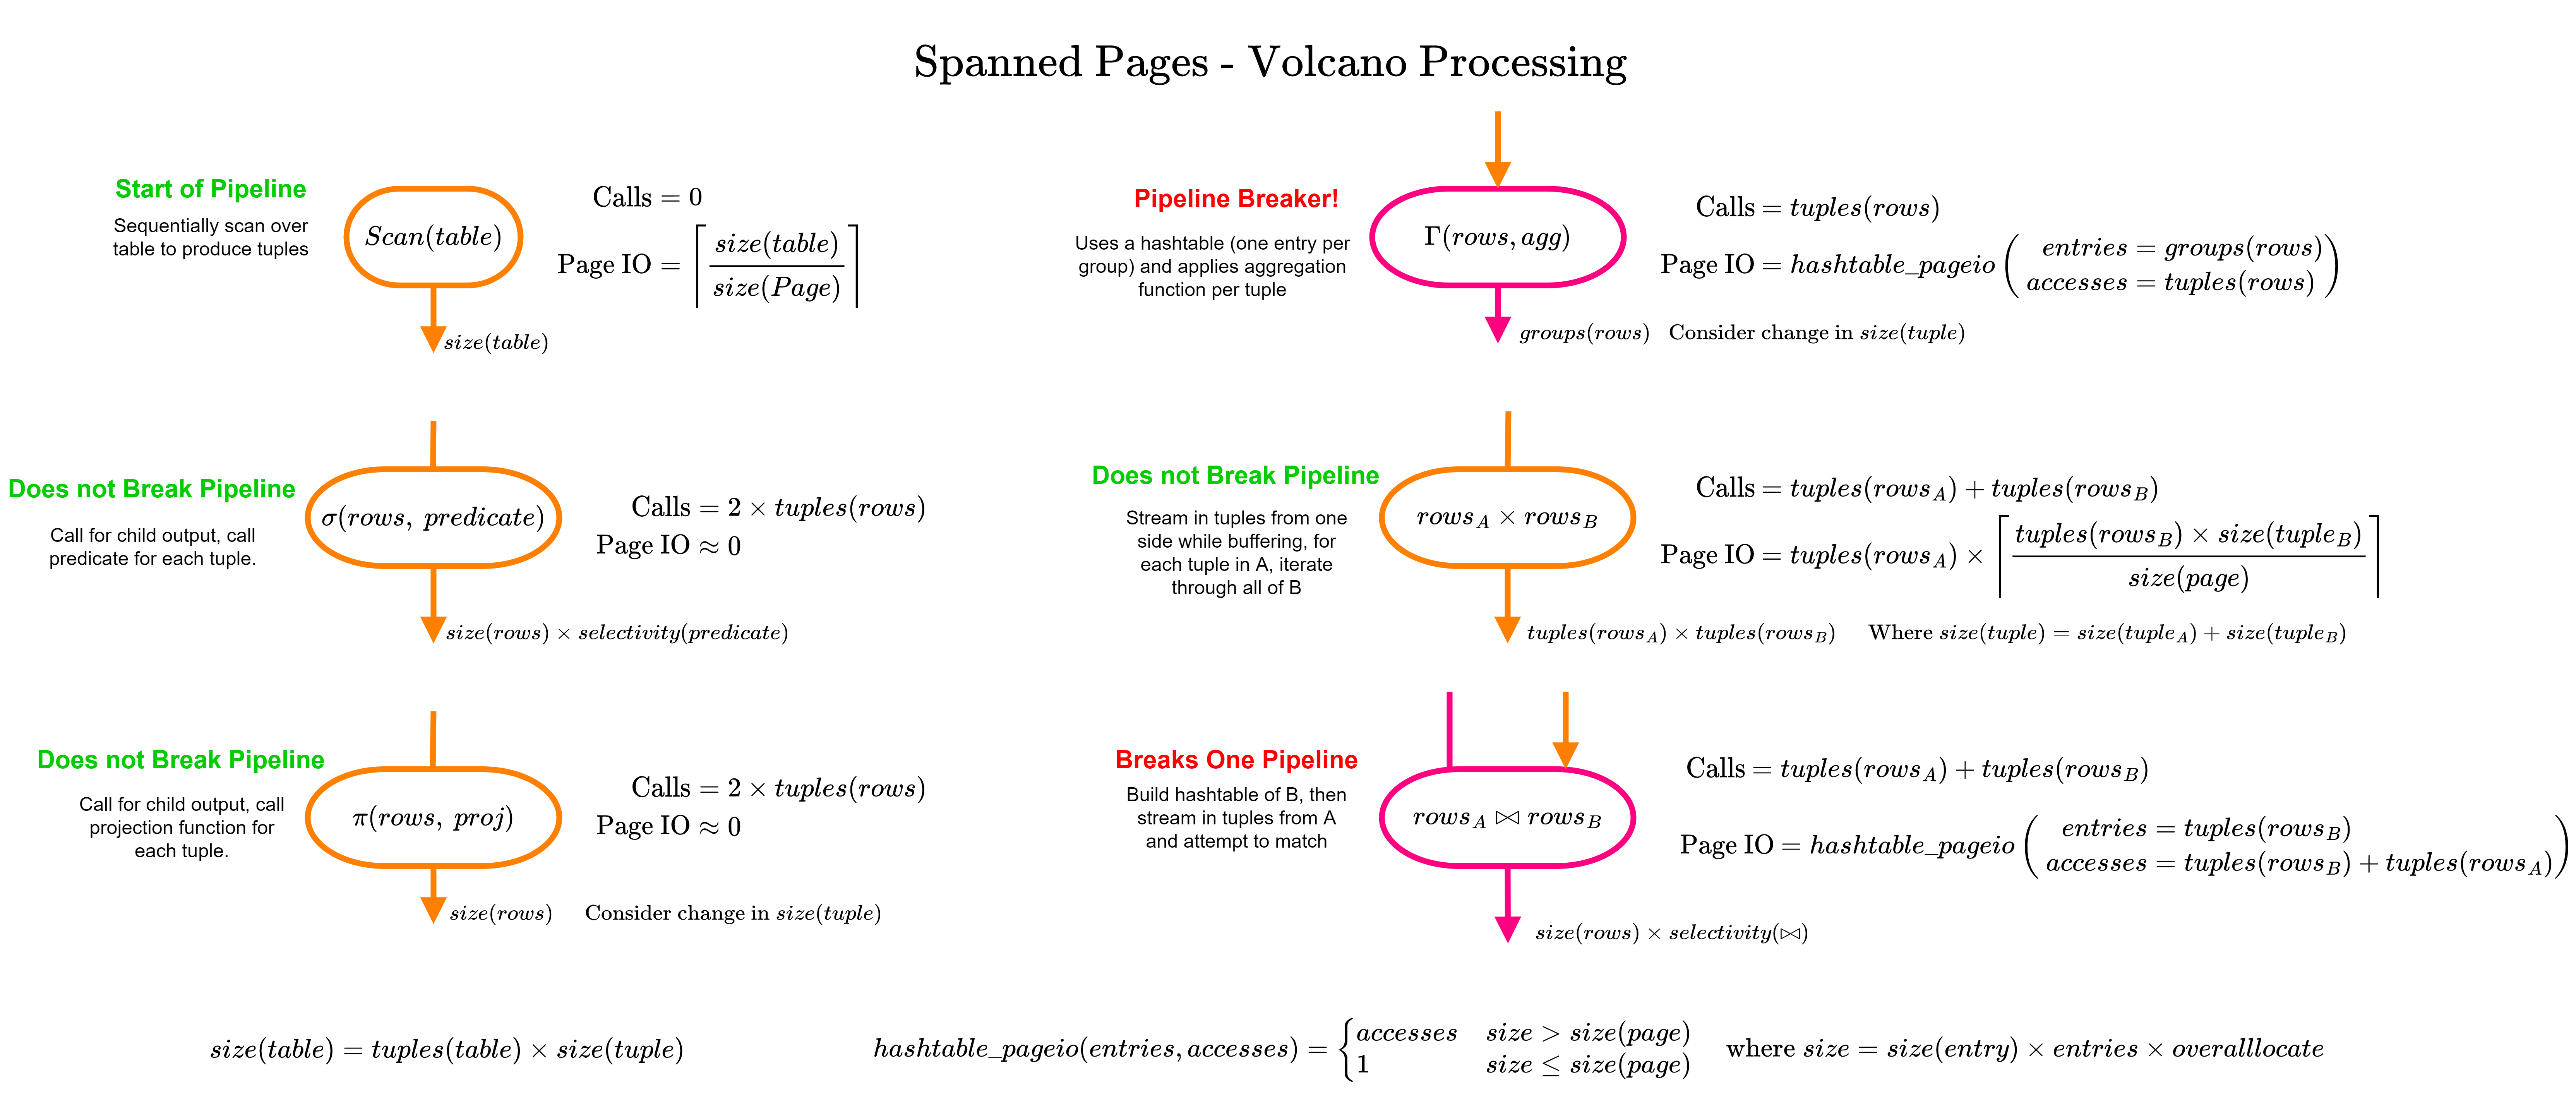
\includegraphics[width=\textwidth]{processing_models/images/spanned_pages_volcano_processing_calcs.drawio.png}
\end{center}

\begin{examplebox}{Selective}
  \begin{minted}{SQL}
CREATE TABLE table (
  a INTEGER,
  b INTEGER,
  c INTEGER
);

-- note a, b and c are uniform randomly distributed [1-16] inclusive 
INSERT INTO table VALUES /* ...10 million rows*/ ;


-- Evaluate the following query for pageIO and function calls under volcano processing.
SELECT sum(c) FROM  table WHERE a = 11 and b = 7;
  \end{minted}
  \tcblower
  If we assume the \mintinline{sql}{WHERE} can be done with a single selection, and selection predicate. 
  \begin{center}
    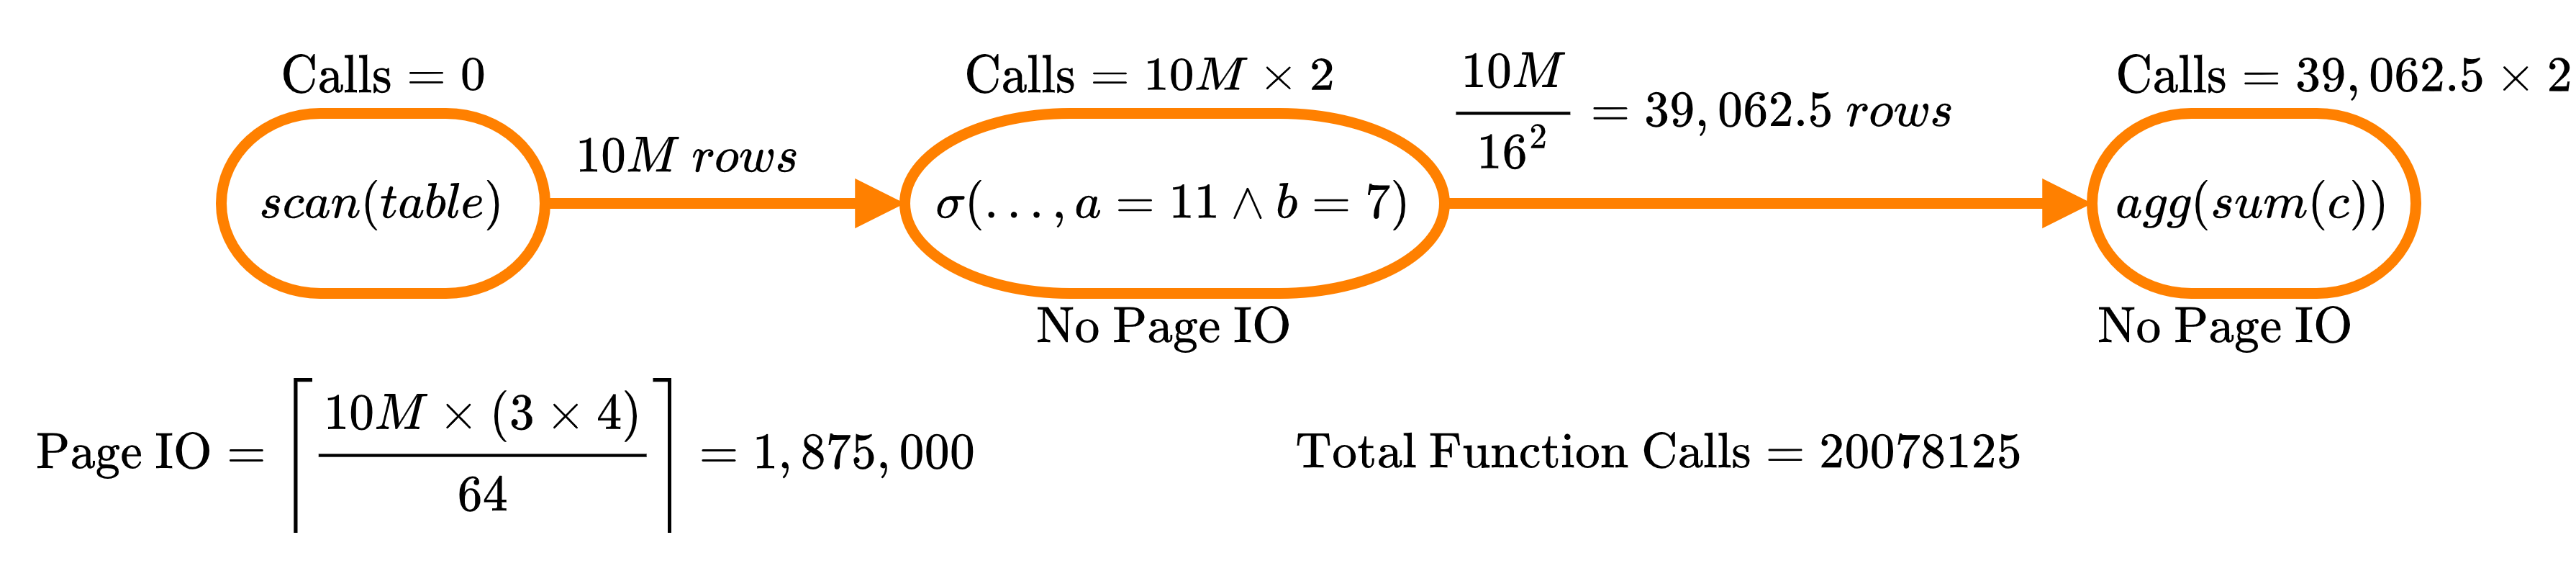
\includegraphics[width=\textwidth]{processing_models/images/example_basic_selection.drawio.png}
  \end{center}
\end{examplebox}

\section{Bulk Processing}
\begin{definitionbox}{Bulk Processing}
  Queries are processed in batches.
  \begin{itemize}
    \item Turn \textit{control dependencies} to \textit{data dependencies} \& buffer.
    \item Pass references to buffers between operators.
    \item Better locality for code (I-cache) \& data.
  \end{itemize}
\end{definitionbox}
For example a basic select operator could be implemented on an Nary Table:
\begin{itemize}
  \item Rather than calling select predicate, provide operators for common predicates (e.g equality)
  \item Can implement for decomposed storage layout.
\end{itemize}
\begin{minted}{cpp}
template <typename V> using Row = vector<V>;
template <typename V> using Table = vector<Row<V>>;

template <typename V>
size_t select_eq(Table<V> &outputBuffer, const Table<V> &inputBuffer, V eq_value, size_t attribOffset) {
  for (const Row<V> &r : inputBuffer) {
    if (r[attribOffset] == eq_value) {
      outputBuffer.push_back(r);
    }
  }
  return outputBuffer.size();
}
\end{minted}
\begin{examplebox}{Bulking up}
  Translate the following to use the \mintinline{cpp}{select_eq} implementation above.
  \begin{minted}{sql}
CREATE TABLE Orders (orderId int, status int, urgency int);

SELECT PendingOrders.* FROM (
  SELECT *
  FROM Orders
  WHERE status = PENDING
) AS PendingOrders
WHERE PendingOrders.urgency = URGENT;
  \end{minted}
  \tcblower
  \begin{minted}{cpp}
enum Urgency { URGENT, NOT_URGENT, IGNORE };
enum Status { COMPLETE, IN_PROCESS, PENDING };

Table<int> Orders{
    {1, COMPLETE, IGNORE},
    {2, PENDING, IN_PROCESS},
    {3, PENDING, URGENT},
    {4, PENDING, URGENT},
};

Table<int> PendingOrders, UrgentAndPendingOrders;

select_eq<int>(PendingOrders, Orders, PENDING, 1);
select_eq<int>(UrgentAndPendingOrders, PendingOrders, URGENT, 2);
  \end{minted}
\end{examplebox}
\noindent
For determining the number of IO operations, bulk operators read all input pages sequentially, and writes to output sequentially.

\begin{examplebox}{Bulk Selection}
  \begin{minipage}{.2\textwidth}
    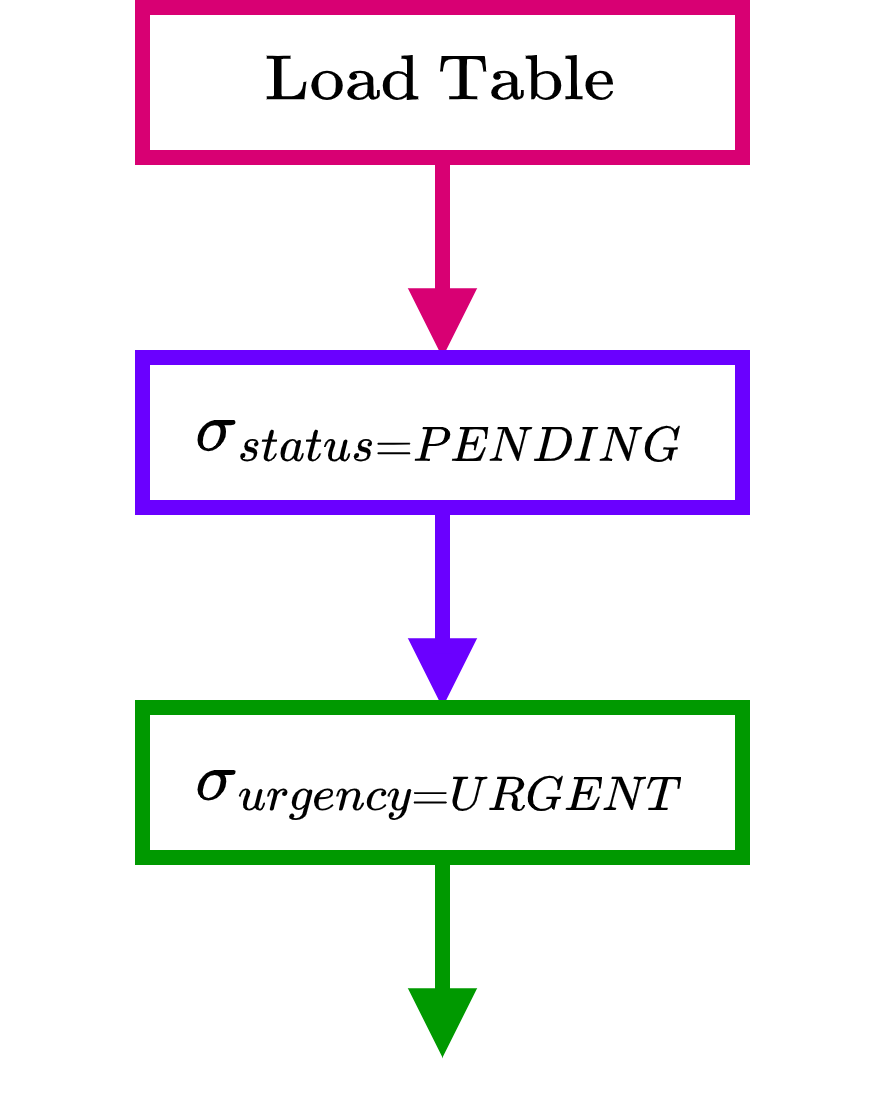
\includegraphics[width=\textwidth]{processing_models/images/example_bulk_processing.drawio.png}
  \end{minipage} \hfill \begin{minipage}{.79\textwidth}
    Compute an estimate of the IO operations for the previous example's query.
    \begin{itemize}
      \item Selectivity of both $\sigma$ is $25\%$
      \item $1,000,000$ tuples
      \item Each tuple contains $3$ $32$ bit integers
      \item $512 \ KB$ cache with $64 \ B$ pages
    \end{itemize}
  \end{minipage}
  \tcblower
  \begin{enumerate}
    \item { Load Page
      \[size(Orders) = 1,000,000 \times (3 \times 4) = 12,000,000 \Rightarrow pages(Orders) = \left\lceil \cfrac{12,000,000}{64} \right\rceil = 187,500 \]
      Hence $187,500$ IO actions
    }
    \item { $\sigma_{status=PENDING}$
      \[size(PendingOrders) = 250,000 \times (3 \times 4) = 3,000,000 \]
      \[\Rightarrow pages(PendingOrders) = \left\lceil \cfrac{3,000,000}{64} \right\rceil = 46,875\]
      Hence given the input buffer, there are $46,875$ output IO actions.
    }
    \item { $\sigma_{urgency=URGENT}$
      \[size(PendingAndUrgentOrders) = 62,500 \times (3 \times 4) = 750,000 \]
      \[\Rightarrow pages(PendingAndUrgentOrders) = \left\lceil \cfrac{750,000}{64} \right\rceil = \lceil 11,718.75 \rceil = 11,719\]
      Hence given the input buffer, there are $11,719$ output IO actions.
    }
  \end{enumerate}
  Hence in total there are $187,500 + 46,875 + 11,719 = 246094$ IO actions.
\end{examplebox}

\subsection{By-Reference Bulk Processing}
\begin{definitionbox}{By-Reference Bulk Processing}
  Copying is expensive, so instead of copying rows an identifier/reference is used.
  \begin{itemize}
    \item There is overhead associated with indirection of a reference
    \item Produced tables can contain many ids out of order \& lookups result in random access pattern.
  \end{itemize}
\end{definitionbox}

\begin{minted}{cpp}
// Candidates are indexes into an underlying table
using Candidates = vector<uint32_t>;

// To add all rows of a table to some candidates.
template<typename V>
size_t add_candidates(const Table<V>& underlyingBuffer, Candidates& outputRows) {
    for (uint32_t i = 0; i < underlyingBuffer.size(); i++) {
        outputRows.push_back(i);
    }
    return outputRows.size();
}

// An by-reference bulk processing implementation of select
template<typename V>
size_t select_eq(const Table<V>& underlyingBuffer, Candidates& outputRows, 
                 const Candidates& inputRows, V eq_value, size_t attribOffset) {
    for (const uint32_t index : inputRows) {
        if (underlyingBuffer[index][attribOffset] == eq_value) {
            outputRows.push_back(index);
        }
    }
    return outputRows.size();
}
\end{minted}
We can then demonstrate the previous example with the following query
\begin{minted}{cpp}
Candidates OrdersCandidates, PendingOrders, UrgentAndPendingOrders;
add_candidates(Orders, OrdersCandidates);
select_eq<int>(Orders, PendingOrders, OrdersCandidates, PENDING, 1);
select_eq<int>(Orders, UrgentAndPendingOrders, PendingOrders, URGENT, 2);
\end{minted}

\subsubsection{Page Access Probability}
When estimating page IO we must consider access to candidates:
\begin{itemize}
  \item Access to candidate vectors can result in page IO.
  \item Indexes from candidate vectors are ordered, but may be spread across the underlying table's pages.
\end{itemize}
Probability of a page being touched, given $s$ selectivity of tuples and $n$ tuples per page.
\[p(s,n) = 1 - \underbrace{(1-s)^n}_{\text{no tuples accessed}}\]
Hence for a selection:
\[PageFault = p(s,n) \times pages(underlying) where \begin{cases}
  s & = \text{ selection selectivity} \\
  n & = \cfrac{\text{page size}}{\text{tuple size}} \\
\end{cases}\]

\subsection{Decomposed Bulk Processing}
Decomposed storage was introduced as a consequence of bulk processing:
\begin{itemize}
  \item By storing columns contiguously, page faults are reduced by accessing a column.
  \item Reduces pressure on space occupied by underlying table in buffer pool/cache (only need relevant columns loaded).
\end{itemize}

\subsubsection{IO Operations}
We must adapt the scheme used for by-reference bulk processing to account of decomposed storage.
\begin{itemize}
  \item Only need to consider the size of the data in the column being accessed.
\end{itemize}
\begin{examplebox}{Bulk Columns}
  \unfinished
\end{examplebox}
